%%%%%%%%%%%%%%%%%%%%%%%%%%%%%%%%%%%%%%%%%%%%%%%%%%%%%%%%%%%%%%%%%%%%%%%%%%%
\chapter{Phase de clôture}
\label{Chapitre_5}
%%%%%%%%%%%%%%%%%%%%%%%%%%%%%%%%%%%%%%%%%%%%%%%%%%%%%%%%%%%%%%%%%%%%%%%%%%%
\section{Introduction}
\label{Introduction}
%%%%%%%%%%%%%%%%%%%%%%%%%%%%%%%%%%%%%%%%%%%%%%%%%%%%%%%%%%%%%%%%%%%%%%%%%%%
Ce chapitre présente la phase de clôture du projet, en mettant l'accent sur la finalisation
technique de la plateforme, les choix d'outils utilisés, ainsi que les résultats obtenus à l'issue
des deux sprints. L'objectif est de synthétiser le travail réalisé et de montrer la cohérence entre
les besoins définis au départ et la solution livrée.




%%%%%%%%%%%%%%%%%%%%%%%%%%%%%%%%%%%%%%%%%%%%%%%%%%%%%%%%%%%%%%%%%%%%%%%%%%%
\section{Environnement technique et outils adoptés}
\label{section5.2}
%%%%%%%%%%%%%%%%%%%%%%%%%%%%%%%%%%%%%%%%%%%%%%%%%%%%%%%%%%%%%%%%%%%%%%%%%%%
Pour concrétiser la plateforme web de gestion de location de véhicules, nous avons retenu
un ensemble d'outils permettant d'assurer la robustesse, la maintenabilité et l'évolutivité de
la solution.

\section{Technologies de développement}
Les technologies utilisées dans ce projet sont présentées dans le tableau suivant:

\begin{table}[!htbp]
\centering
\caption{Technologies utilisées}
\label{tab:technologies-utilisees}
\renewcommand{\arraystretch}{1.3}
\begin{tabular}{|l|p{10.2cm}|}
\hline
\textbf{Technologie} & \textbf{Description} \\
\hline

\includegraphics[height=0.7cm]{Chapitres/Figures/Laravel-Logo.png}\hspace{0.2cm}Laravel & Framework PHP utilisé pour développer le backend et exposer les API REST. \\
\hline

\includegraphics[height=0.7cm]{Chapitres/Figures/React-logo.png}\hspace{0.2cm}React & Bibliothèque utilisée pour construire l'interface utilisateur côté client. \\
\hline

\includegraphics[height=0.7cm]{Chapitres/Figures/Mysql-logo.png}\hspace{0.2cm}MySQL & Système de gestion de base de données relationnelle du projet. \\
\hline

\includegraphics[height=0.7cm]{Chapitres/Figures/vite-logo.png}\hspace{0.2cm}Vite & Outil de build et serveur de développement pour le frontend. \\
\hline

\includegraphics[height=0.7cm]{Chapitres/Figures/Tailwind-logo.png}\hspace{0.2cm}Tailwind CSS & Framework CSS utilitaire utilisé pour styliser rapidement l'interface. \\
\hline
\end{tabular}
\end{table}


%%%%%%%%%%%%%%%%%%%%%%%%%%%%%%%%%%%%%%%%%%%%%%%%%%%%%%%%%%%%%%%%%%%%%%%%%%%
\section{Logiciels utilisés}
\label{section5.3}
%%%%%%%%%%%%%%%%%%%%%%%%%%%%%%%%%%%%%%%%%%%%%%%%%%%%%%%%%%%%%%%%%%%%%%%%%%%
Les logiciels utilisés dans le cadre de ce projet sont présentés dans le tableau suivant:

\begin{table}[!htbp]
\centering
\caption{Logiciels utilisés}
\label{tab:logiciels-utilises}
\renewcommand{\arraystretch}{1.3}
\begin{tabular}{|l|p{10.2cm}|}
\hline
\textbf{Technologies} & \textbf{Description} \\
\hline

\includegraphics[height=0.7cm]{Chapitres/Figures/lucid-logo.png}\hspace{0.2cm}Lucidchart & Outil de modélisation UML utilisé pour les diagrammes de conception. \\
\hline

\includegraphics[height=0.7cm]{Chapitres/Figures/vscode-logo.png}\hspace{0.2cm}Visual Studio Code & Editeur de code utilisé pour le développement de l'application web. \\
\hline

\includegraphics[height=0.7cm]{Chapitres/Figures/overleaf-logo.png}\hspace{0.2cm}Overleaf (LaTeX) & Plateforme de rédaction utilisée pour la préparation du rapport. \\
\hline

\includegraphics[height=0.7cm]{Chapitres/Figures/teams-logo.png}\hspace{0.2cm}Microsoft Teams & Outil de visioconférence utilisé pour les réunions et les échanges à distance. \\
\hline

\includegraphics[height=0.7cm]{Chapitres/Figures/XAMPP-logo.png}\hspace{0.2cm}XAMPP & Environnement local regroupant Apache et PHP pour l'exécution et les tests de l'application. \\
\hline

\includegraphics[height=0.7cm]{Chapitres/Figures/phpmyadmin-logo.png}\hspace{0.2cm}phpMyAdmin & Interface web de gestion de la base de données MySQL. \\
\hline

\includegraphics[height=0.7cm]{Chapitres/Figures/github-logo.png}\hspace{0.2cm}Git/GitHub & Outils de gestion de versions et de collaboration sur le code source. \\
\hline
\end{tabular}
\end{table}




%%%%%%%%%%%%%%%%%%%%%%%%%%%%%%%%%%%%%%%%%%%%%%%%%%%%%%%%%%%%%%%%%%%%%%%%%%%
\section{Mise en production et organisation du déploiement}
\label{section5.4}
%%%%%%%%%%%%%%%%%%%%%%%%%%%%%%%%%%%%%%%%%%%%%%%%%%%%%%%%%%%%%%%%%%%%%%%%%%
La phase de déploiement a consisté à préparer une version stable de l'application,
incluant la configuration des variables d'environnement, la sécurisation des accès
et la vérification du bon fonctionnement des modules principaux.

Une attention particulière a été portée à:
\begin{itemize}
	\item la cohérence entre les environnements de développement et d'exécution,
	\item la fiabilité des échanges entre frontend et backend,
	\item la validation finale des fonctionnalités métier (réservation, réclamations,
	statistiques et messagerie).
\end{itemize}




	%%%%%%%%%%%%%%%%%%%%%%%%%%%%%%%%%%%%%%%%%%%%%%%%%%%%%%%%%%%%%%%%%%%%%%%%%%%
	\section{Choix technologiques}
	\label{sec:choix-technologiques}
	%%%%%%%%%%%%%%%%%%%%%%%%%%%%%%%%%%%%%%%%%%%%%%%%%%%%%%%%%%%%%%%%%%%%%%%%%%%

	\subsection{Architecture retenue dans notre projet}
	Dans notre application, nous avons adopté une architecture API Laravel (backend)
	+ SPA React (frontend). Le backend suit principalement une logique MVC enrichie
	par une couche Service, afin de séparer clairement les responsabilités et de
	faciliter la maintenance.

	\begin{itemize}
		\item \textbf{Modèle (Model)}: gère les entités métier et l'accès aux données
		(utilisateurs, agences, véhicules, réservations, paiements, etc.). Les modèles
		représentent la structure des données et les relations entre entités.

		\item \textbf{Contrôleur (Controller)}: reçoit les requêtes HTTP, orchestre le
		traitement et renvoie la réponse. Dans notre projet, les contrôleurs sont
		volontairement légers: ils délèguent la logique métier aux services et
		s'appuient sur une gestion centralisée des erreurs.

		\item \textbf{Vue}: dans une API REST, la « vue » est remplacée par des réponses
		JSON standardisées. Côté client, c'est l'interface React qui joue le rôle
		d'affichage et d'interaction utilisateur.
	\end{itemize}
	
\begin{figure}[H]
\centering
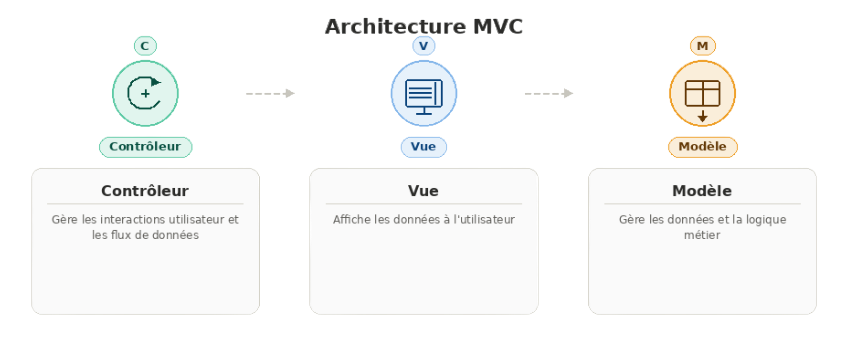
\includegraphics[width=0.9\textwidth]{Chapitres/Figures/diag_mvc.png}
\caption{Architecture MVC}
\label{fig:diag-mvc}
\end{figure}

\subsection{Diagramme de déploiement}
<<Un diagramme de déploiement fait partie de la catégorie des diagrammes structurels, car il décrit un aspect du système même. Dans le cas présent, le diagramme de
déploiement décrit le déploiement physique des informations générées par le logiciel sur
des composants matériels.>> \cite{lucidchart-deploiement}

\begin{figure}[H]
\centering
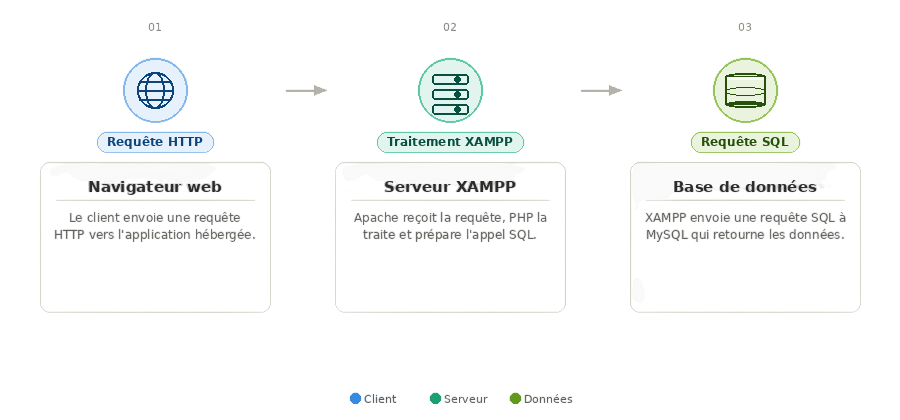
\includegraphics[width=0.95\textwidth]{Chapitres/Figures/diag_deploiement.png}
\caption{Diagramme de déploiement}
\label{fig:diag-deploiement}
\end{figure}

\subsection{Diagramme de Gantt}
Le diagramme de Gantt ci‑dessous récapitule les principales phases et tâches du projet, telles qu'elles ont été réalisées durant la période du 02/02/2026 au 15/05/2026.

\begin{table}[!htbp]
\centering
\caption{Diagramme de Gantt}
\label{tab:diagramme-gantt}
\renewcommand{\arraystretch}{1.3}
\resizebox{\textwidth}{!}{%
\begin{tabular}{|c|p{7.8cm}|c|c|c|}
\hline
\textbf{ID} & \textbf{Nom de tâches} & \textbf{Date début} & \textbf{Date fin} & \textbf{Durée} \\
\hline
1 & Auto-formation & 02/02/2026 & 12/02/2026 & 15 jours \\
\hline
2 & Étude et planification du projet & 13/02/2026 & 28/02/2026 & 17 jours \\
\hline
3 & Sprint 01 — Gérer des intervenants & 01/03/2026 & 21/03/2026 & 28 jours \\
\hline
4 & Sprint 02 — Gérer des processus des réservations & 01/04/2026 & 23/04/2026 & 29 jours \\
\hline
5 & Liaison et clôture & 01/05/2026 & 10/05/2026 & 10 jours \\
\hline
6 & Rédaction du rapport & 02/02/2026 & 11/05/2026 & 99 jours \\
\hline
\multicolumn{4}{|r|}{\textbf{Période couverte}} & \textbf{02/02/2026 -- 11/05/2026} \\
\hline
\end{tabular}%
}
\end{table}

\begin{figure}[H]
\centering
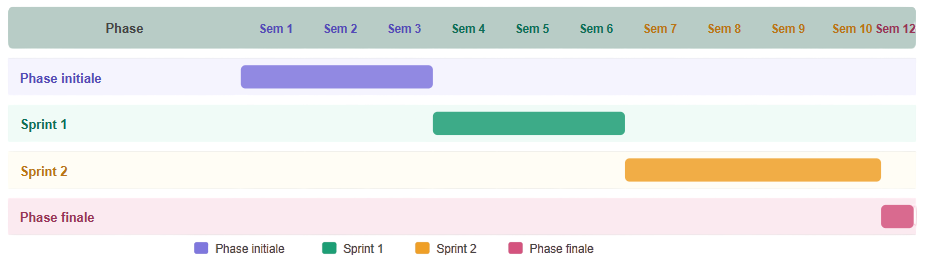
\includegraphics[width=0.95\textwidth]{Chapitres/Figures/gantt.png}
\caption{Diagramme de Gantt}
\label{fig:gantt-image}
\end{figure}

%%%%%%%%%%%%%%%%%%%%%%%%%%%%%%%%%%%%%%%%%%%%%%%%%%%%%%%%%%%%%%%%%%%%%%%%%%%
\section{Conclusion}
%%%%%%%%%%%%%%%%%%%%%%%%%%%%%%%%%%%%%%%%%%%%%%%%%%%%%%%%%%%%%%%%%%%%%%%%%%%
En conclusion, ce chapitre a permis de formaliser la phase finale du projet en présentant
les outils mobilisés, les choix techniques retenus et les résultats atteints. Cette étape confirme
la cohérence entre la planification initiale et la solution réalisée, tout en ouvrant la voie
à des améliorations futures de la plateforme.



